\chapter{Marco Teórico - (In) Seguridad en el Browser}
\label{chap3:MT}

En esta sección se presentan los posibles ataques que un \textit{Browser} puede sufrir y que directamente podrían afectar al sistema con el que se comunica. Principalmente ahondaremos en los ataques en el \textit{Browser} relacionados a las técnicas de Ingeniería Social \cite{socEngineeering}. El escenario actual de los ataques en el \textit{browser} ha cambiado bastante, si es comparado a aquellos de la decada de los noventa. Cada día los Browsers son más robustos y difíciles de explotar, y por lo mismo los ataques de tipo \textit{drive-by downloads} o los basados en ejecución de código para vulnerar el sistema, cada vez son menores. Una nueva forma de ataque ha emergido y es bastante fácil de lograrlo, pues se basa en el engaño del usuario a realizar lo que el atacante desea. Una vez el usuario es engañado, el atacante puede lograr un control total tanto del \textit{Browser} o del Host, sin haber tenido que vulnerar el sistema \cite{Rajab2013,Labs2013} que aloja al \textit{Browser}. Desarrollos de sistemas críticos que interactuan a diario con diferentes usuarios en la red, deberían de ser los más preocupados de estos ataques pues atentan contra la confidencialidad, integridad y disponibilidad de los datos, tanto del usuario (personales) como los de los \textit{Stakeholders} involucrados.

\section{Social Engineering o Ingeniería Social}
\cite{socEngineeering} define este tipo de acción como: El acto de manipular una persona para realizar acciones que no son parte de los mejores intereses del \textit{blanco o víctima} (la misma persona/organización/etc u otra entidad). Un ataque de éste tipo puede darse de diversas maneras, no dejando la posibilidad de un encuentro físico o digital con el que realiza el engaño. Un ataque basado en ingeniería social, es uno que se aprovecha del comportamiento humano y la confianza de la víctima. En el contexto del Web Browser, el usuario engañado es la primera y última línea de defensa contra este tipo de ataques, pues un abuso en la confianza del usuario podría abrir las puertas al Host del \textit{Browser}, logrando un daño tanto del usuario como con los sistemas externos con los que interactúa.

Si pudieramos dividir los ataques de Social Engineering, podríamos encontrarnos con un panorama parecido al de la Figura \ref{fig:SEattack}. En esta figura es posible observar que los ataques de Clickjacking se encuentran afuera del ámbito de los ataques de  Ingeniería Social, esto es dado a que el usuario que está navegando, pudo haber accedido a una página web conocida por él, sin siquiera que el atacante haya sugestionado a éste. Sin embargo, Clickjacking puede terminar convirtiendose en un ataque de Social Engineering si se combina con otros procedimientos.

	\begin{figure}[h!t]
        \centering
        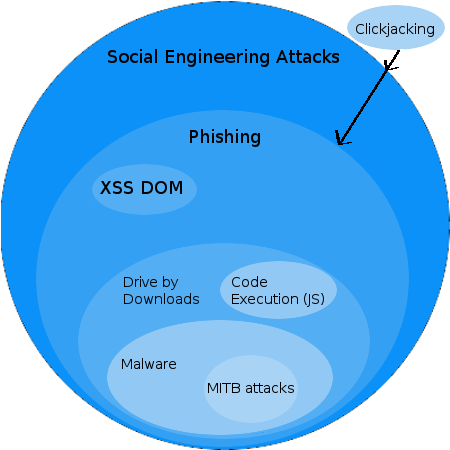
\includegraphics[scale=0.5]{figures/SEAttacks.png}
        \caption{Esquematización de ataques de tipo Social Engineering. Fuente: Elaboración Propia.}
        \label{fig:SEattack}
    \end{figure}

 	\subsection{Análisis de ataques}
	Según los estudios \cite{browSecPhish, Labs2013, rowSecSEMBlock} indican que el \textit{Browser} es la primera linea de defensa en contra de multiples amenazas en la Web. Sin embargo, esto se ve afectado bastante por la falta de educación de los usuarios que utilizan los navegadores y la constante evolución de las amenazas \cite{browSecPhish} Es por esto que muchos de los manufacturadores de browsers crean mecanismos de defensa \cite{Drake2011} que actuen al momento de solicitar una página, usando black o white list, sistemas de reputación \cite{Rajab2013} con avisos de alerta al usuario, para evitar que éste al menos tome la decisión de poder ingresar al sitio malicioso.

\section{Ataques y Amenazas}
Esta sección incluye algunos ataques posibles de realizar en un \textit{Browser} y que podrían afectar tanto directa como indirectamente a un sistema externo. Acá no incluiremos ataques en donde el Host ya ha sido vulnerado con anticipación, o aquellos que puedan correr software con los privilegios de un usuario del sistema Host, es decir, aquellos donde el Host ya ha sido controlado directamente por medio de alguna vulnerabilidad del sistema. En el caso anterior, los Browsers ya nada pueden hacer para detener un ataque de esa magnitud.

En el Top Ten \cite{owaspTopTen} de la OWASP (Open Web Application Security Project) - los diez riesgos de seguridad más importantes en Aplicaciones Web - se puede distinguir en el año 2013 los riesgos directamente relacionados a amenazas de seguridad en el \textit{Browser}. Algunos como: Injección (A1), Manejo de sesiones y autenticación roto (A2), XSS (A3) y uso de componentes con vulnerabilidades conocidas (A9), son los riesgos que las organizaciones podrían sufrir en sus sistemas cuando se realizan ciertos ataques en el \textit{Browser}.

En trabajos \cite{barth2008security, FirefoxThreatModel} se puede observar que existen ataques que pueden generar secuelas en otros sistemas, si es que el Navegador es afectado en primera instancia. Algunas amenazas existentes son:

\begin{enumerate}
	\item Compromiso de los componentes del Navegador (plugins incluídos) que poseen privilegios de usuario.
	\item Compromiso del Host/Sistema.
	\item Robo de datos en el tráfico.
	\item Compromiso de páginas web (y su data) de origenes distintos.
	\item Fijación de sesión o robo de ésta.
	\item Compromiso de los canales de comunicación del \textit{Browser}.
\end{enumerate}

Una lista (parcial) de ataques asociados a las amenazas anteriores son:

\subsection{Phishing}
Este ataque consta principalmente del engaño al usuario, confundiendolo a que visite una página deshonesta en vez de la que tenía pensado; es uno de los tantos ataques que usan la ingeniería social para dañar a un usuario. En el estudio realizado por NSS Labs \cite{browSecPhish} afirma que muchos de los ataques que actualmente están ocurriendo se han limitado al uso de técnicas de ingeniería social. Si bien los ataques basados en drive-by downloads y clickjacking siguen siendo de alto impacto, los atacantes parecen preferir los otros por la simplicidad de éste, pues no es necesario conocer realmente vulnerabilidades del \textit{Browser} para llevarlos a cabo. 


	\subsubsection{Instalación de Malware o Extensiones malignas}
	Un ataque de este tipo puede ser originado desde la ejecución de un ataque Phishing a una persona; en especial cuando se hace creer que lo que se va a instalar es completamente inofensivo. Sin embargo, el resultado de la aceptación de usuario a la instalación puede tener consecuencias bastante graves tanto en el Browser como en el Host, donde la mayoría de las veces el ataque puede terminar como un Man-in-the-Browser \cite{Utakrit2009, Dougan2012}. 

	\subsubsection{Extensiones vulnerables}
	Muchas veces un ataque Phishing se aprovechará de las extensiones \textit{benign-but-buggy}, es decir, de extensiones que tienen un propósito benigno para el usuario que las usa, pero que un atacante puede aprovecharse de alguna vulnerabilidad \cite{Barth2010, Liu2012}. Además dependiendo del tipo de arquitectura que el Browser pueda tener, es posible que el atacante utilice una extensión que tenga permisos a ciertos recursos del Host o que pueda coludirse con otra extensión benigna para lograr un ataque en forma conjunta \cite{Saini2014}; donde lo peor de todo, es que el tráfico no será detectado como malicioso.

	\subsubsection{Ejecución de Código Javascript}
	En ciertas situaciones un atacante podría aprovecharse de alguna vulnerabilidad asociada a los modelos de seguridad que Javascript y DOM poseen, pues ambos son totalmente transversales. Javascript utiliza un modelo de seguridad en sus objetos basado en \textbf{Capabilities}, mientras que DOM refuerza el \textbf{Same Origin Policy} por medio del uso de un \textbf{Reference Monitor} para controlar el acceso de código de diversos \textbf{orígenes}. Es en esta situación donde podría llevarse a cabo la ejecución de código javascript aún cuando éste pueda ser de un \textbf{origen} distinto al receptor \cite{Barth2009}.

	\subsubsection{XSS - Cross-Site Scripting DOM}
	El ataque Cross-Site Scripting (XSS) normalmente se asocia con ataques que afectan directamente al servidor, pero existe una tercera variedad que afecta directamente al navegador \cite{Singh2014} y que puede ser tan peligrosa como su forma \textit{Reflajada} o \textit{Almacenada}, esta es llamada XSS DOM o \textbf{tipo-0 XSS} \cite{XSSDOMOwasp, XSSDOM}. Es un ataque XSS en donde su \textit{payload} de ataque es ejecutado como resultado de la modificación del \textit{ambiente} DOM en el navegador de la víctima usado por el código script original; en consecuencia el código de cliente se ejecuta de una manera inesperada. Un ejemplo de un simple XSS DOM puede verse en \cite{bugzillaXSSDOM}. Un UXSS o Universal XSS es un ataque más particular, y tiene la habilidad de ser gatillado al explotar una falla en el interior del Browser \cite{Paola2006}, a diferencia de otros XSS que buscan la vulnerabilidad dentro del Servidor Web al que se comunican.


	\subsubsection{Man in the \textit{Browser} (MitB)}
	La diferencia sustancial entre un Man in the Browser (MitB) y un Man in the Middle (MitM) es el dominio que ataca, el primero es al nivel de la capa de aplicación, mientras que el segundo tiene que ver más con el canal de comunicación. \cite{Dougan2012} explica las grandes diferencias entre estos dos ataques, donde principalmente un MitB se inicia con un ataque Phishing que logra convencer al usuario de instalar alguna extensión o ejecutar una pieza de código \cite{Utakrit2009, Paola2006}, que permita al atacante estar entre el Browser y el Host, de tal manera que todas las solicitudes puedes ser escuchadas y modificadas dentro del mismo Host.



%\section{Mecanismos de Defensa del Host}
%	Dependiendo del Sistema Operativo, es posible encontrar diversos mecanismos de Defensa. Tanto Linux como Windows poseen mecanismos parecidos, donde se diferencia la implementación. Dado que la mayor parte de los usuarios en internet usan Windows (Figura \ref{fig:OS}) nos enfocaremos en éste para mostrar los mecanismos implementados en el Host.

%	\begin{figure}[h!t]
 %       \centering
  %      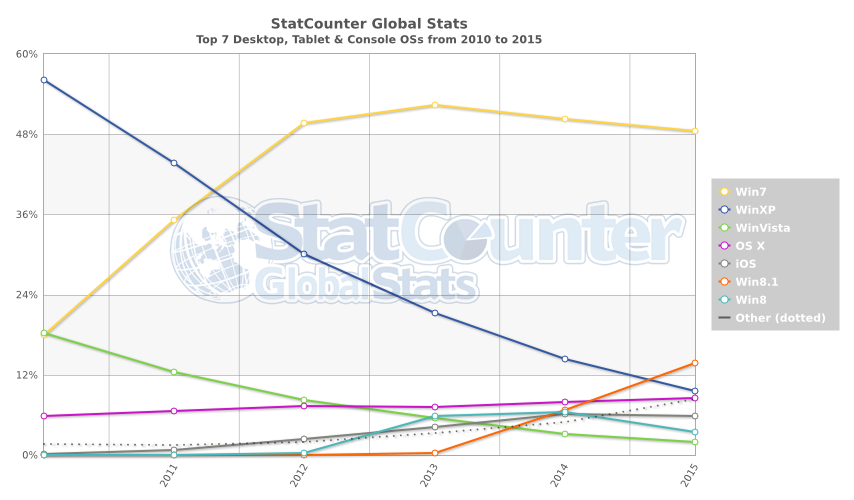
\includegraphics[scale=0.5]{figures/StatCounter-os-ww-yearly-2010-2015.png}
   %     \caption{Gráfico con porcentaje de tipo de sistemas operativos más usados. Fuente: \cite{statOS}}
    %    \label{fig:OS}
    %\end{figure}

    %\subsection{DEP/NX o Data Execution Prevention}

    %\subsectiob{ASLR o Address Space Layout Randomization}

    %\subsection{/GS (Buffer Security Check)}

    %\subsection{SafeSEH}

    %\subsection{Function Pointer Ofuscation}

    %\subsection{Export Address Table Access Filtering (EAF)}

    %\subsection{NULL page allocation}

\section{Mecanismos de Defensa del \textit{Browser}}

\subsection{Sandboxing de procesos/componentes}
    \label{chap3:Sandboxing}
    La idea es encapsular el área de mayor probabilidad de ataque en un espacio aislado, minimizando la superficie de ataque de un software. Sandboxing no es una técnica tan nueva, han existido sistemas que ya lo han incorporado. Ésta protección puede ser aplicada dependiendo del diseño del software, algunos ocupan Sandbox a nivel del sistema operativo como otros que ocupan al nivel del \textit{engine} de Javascript \cite{reis2009browser}. En el caso especial del \textit{Browser}, esta técnica es construida en el nivel más alto posible para un programa de usuario, lo que permite la separación de privilegios entregados por el sistema operativo al \textit{browser} y los subprocesos que corren dentro de éste. El atacante que se enfrente a un \textit{browser} que tenga este mecanismo de defensa, tendrá que realizar primero un \textit{bypass} encontrando una vulnerabilidad en el sandboxing del \textit{browser}. Existen diferentes técnicas para Sandboxing, todo depende del diseño del \textit{Browser}.

    En el desarrollo de \cite{barth2008security} se define un modelo de amenazas donde se enumeran las habilidades que debería de tener un atacante y los objetivos de estos, para así caracterizar y evaluar las propiedades de seguridad necesarias para evitar que los atacantes cumplan su objetivo. Una propiedad importante que hacen destacar en el estudio es cómo aislar ciertos procesos que pueden ser aprovechados por los atacantes y ofrece una forma para poder mitigar esto: Sandboxing. El Sandboxing de Google Chrome previene al atacante de leer o escribir en el sistema de archivos del usuario, dejando al Principal Web con los privilegios necesarios para parsear un HTML/XML y ejecutar código JavaScript. Sin embargo esta arquitectura no imposibilita al atacante a atacar otros sitios web si es que el Rendering Engine fue comprometido, lo que puede convertirse en una amenaza muy grande para otros sitios web.

    Mientras Google Chrome e Internet Explorer utilizan un Sandbox para sus procesos de Renderizado \cite{sandboxGC, }, Firefox no ha realizado este trabajo siquiera en su versión monoproceso \cite{NeckoElectro}.

 \subsection{Aislación de contenido}
 	\textbf{Origen} debe ser aislado entre cada página renderizada.
 	%Firefox: FirefoxThreatModel,
 	%GC: Barth2010, Barth2009SecureFrame, Reis2009, barth2008security
 	%IE: Crowley2010, Yason
 	%Todo: Drake2011, Saini2014, Silic2010

 	\subsubsection{En contenido}

 	\subsubsection{En extensiones}

 \subsection{Blacklist y Whitelist de sitios web}
 	\subsubsection{Safe Browsing}
 		%GC y Firefox
 	\subsubsection{SmartScreen}
    %\cite{Crowley2010, Colvin2010}Smartscreen

 \subsection{Sistemas de Reputación - basados en CAMP}
 	%Agregar que estos s complementar con blacklist y a veces whitelist (GC)
 	\subsubsection{Google Download - Google Chrome/Chromium}
 		%Ocupar referencias de NSS para los resultados obtenidos
 	\subsubsection{SmartScreen - Internet Explorer}

 \subsection{Filtros XSS}
 	%Google e IE
 	%Firefox ocupa 3rd party
 	%Vulnerabilidades mencionadas \cite{Bates2010}y la solución del paper es crear un filtro que detenga los ataques antes de que sean interpretados por el Renderer
 \subsection{Safe Sanitization}

 \subsection{AdBlocker}

 \subsection{Actualizaciones Periódicas en Background}


 
